\documentclass[11pt,a4paper]{article}
\usepackage[utf8]{inputenc}
\usepackage{amsmath, amssymb, amsthm}
\usepackage{geometry}
\usepackage{fancyhdr}
\usepackage{hyperref}
\usepackage{graphicx}
\usepackage{enumitem}
\usepackage{color}
\usepackage{titlesec}
\usepackage{enumerate}

% Set the page geometry
\geometry{a4paper, margin=1in}

% Customize the header and footer
\pagestyle{fancy}
\fancyhf{}
%\fancyhead[L]{\textbf{Lecture Title}}
%\fancyhead[R]{\textbf{Date}}
\fancyfoot[C]{\thepage}

% Title format
\titleformat{\section}
  {\normalfont\Large\bfseries}{\thesection}{1em}{}
\titleformat{\subsection}
  {\normalfont\large\bfseries}{\thesubsection}{1em}{}

% Define theorem styles
\newtheorem{theorem}{Theorem}[section]
\newtheorem{definition}[theorem]{Definition}
\newtheorem{lemma}[theorem]{Lemma}
\newtheorem{corollary}[theorem]{Corollary}
\newtheorem{proposition}[theorem]{Proposition}
\newtheorem{example}[theorem]{Example}

% Custom commands
\newcommand{\R}{\mathbb{R}}
\newcommand{\N}{\mathbb{N}}
\newcommand{\Z}{\mathbb{Z}}
\newcommand{\Q}{\mathbb{Q}}
\newcommand{\C}{\mathbb{C}}
\newcommand{\E}{\mathbb{E}}
\newcommand{\Var}{\text{Var}}

\begin{document}

\title{Lecture Notes on Lee-Yang zeros}
\author{Simran Singh}
\date{23 May 2024}
\maketitle

\tableofcontents
\newpage

\section{Introduction}
Lee \& Yang in 1952, gave us a new way to look for phase transitions. Their idea was to consider the \emph{complex zeros} of the grand canonical partition function and study how these zeros behave when varying parameters like external magnetic field, chemical potential and temperature (whichever is applicable) in the system. The main motivation to look at such zeros is because thermodynamic functions can be expressed as logarithms of the partition function and it's derivatives, in which case these functions will develop non-analyticities. In order to make this discussion more rigorous we will first consider some important theorems developed by Lee \& Yang. Following this we will see how the location and trajectory of these zeros can help us determine the location and order of the phase transition. We will finally go back to the Ising model and use the exact result derived for the $1$D Ising model in the previous lecture to verify the \emph{Circle theorem}.

\section{Lee-Yang and Circle theorems}

\begin{theorem}
For all positive real values of $z$, the quantity
\begin{equation}
    f(z) = \lim_{V \to \infty} \frac{1}{V} \log Z^V_{GC}(z)
\end{equation}
approaches a limit that is independent of the shape of $V$\footnote{An assumption is made about the surface area to volume ratio of the shape of V. The surface surface area cannot increase faster than $V^{2/3}$}. Moreover, this limit is a continuous, monotonically increasing function of z.
\end{theorem}

\begin{theorem}
If in the complex z plane a region R containing a segment of the positive real axis is always free of roots, then in this region as $V \to \infty$ all the quantities
\begin{equation}
    \frac{1}{V} \log Z^V_{GC}(z) \,\,, \, \left(\frac{\partial}{\partial \log z}\right) \frac{1}{V} \log Z^V_{GC}(z) \,\,,\, \left(\frac{\partial}{\partial \log z}\right)^2 \frac{1}{V} \log Z^V_{GC}(z)
\end{equation}
approach limits which are analytic with respect to z. Furthermore, the operations $\frac{\partial}{\partial \log z}$ and $\lim V \to \infty$ commute in R.
\end{theorem}

In the following, we will explain how the theorems mentioned above relate to phase transitions and the associated non-analyticities of the partition function. It is ultimately the form of the region $R$ that decides whether a phase transition occurs in a system. If there exists a region $R$ that includes the entire positive real axis (in $z$) such that it is free of any roots of $Z_{GC}$, then all the quantities depending on $\log Z_{GC}$ will be analytic at all real values of $\log z$ and we conclude that our system exhibits no phase transitions (our system exists in a single phase throughout $R$). If, on the other hand, the zeros of the partition function, with increasing volume of the system, close-in on the real axis at, say, at a point $z_1$, then this point divides the real axis into two parts $R_1$ and $R_2$ separated by the point $z_1$. At this point, the quantities depending on $Z_{GC}$ will display non-analyticities (in the form of discontinuity or multi-valuedness). The conclusion in this situation is that the system undergoes a phase transition at $z_1$ and divides the phase space into two regions $R_1$ and $R_2$ both of which are single phases (see Fig. \ref{fig:LYTHEM}).

The nature of the phase transition is further decided by the manner in which the zeroes of the partition function close-in on (or approach the real positive $z$ axis). A first order transition occurs when the Lee-Yang zeros cross the positive real z axis at the phase transition point. Whereas, a second order transition occurs when complex conjugate pairs of poles “pinch” the axis in the $V \to \infty$ limit (see Fig. \ref{fig:LYEVinft}).

\begin{figure}[ht]
    \centering
    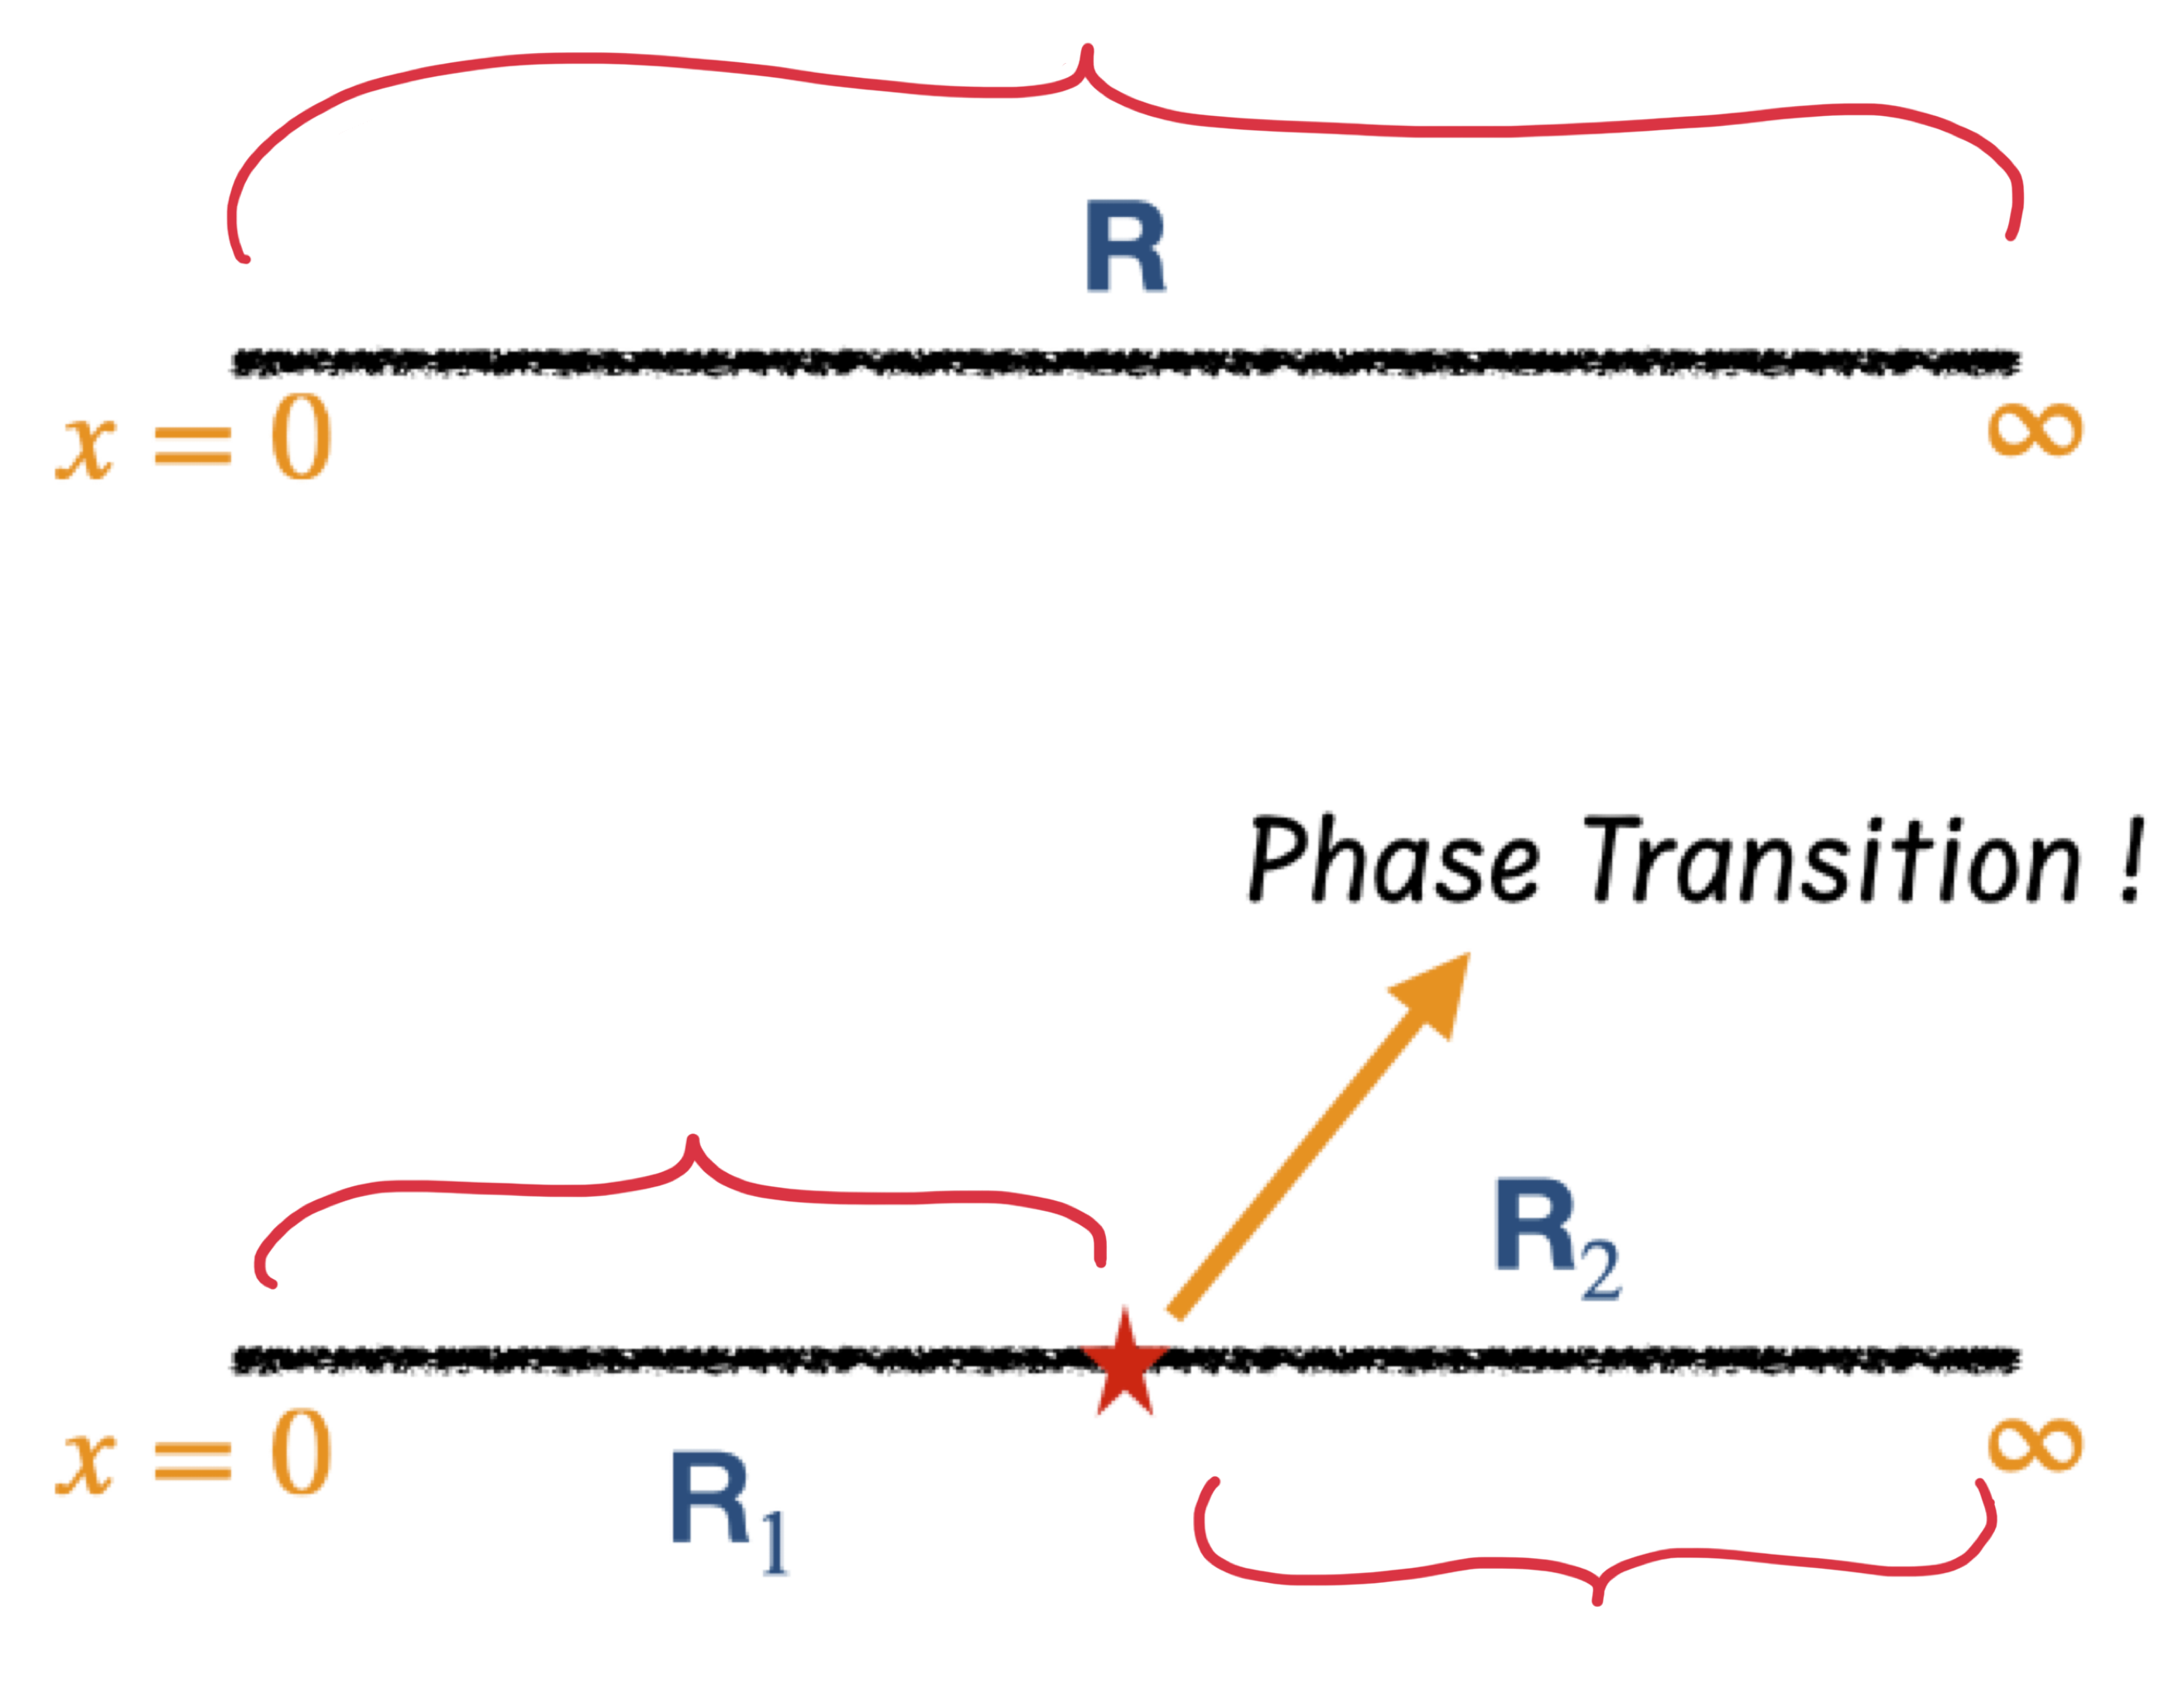
\includegraphics[scale=0.075]{LYTheorem.png}
    \caption{Yang-Lee theorems in a nutshell}
    \label{fig:LYTHEM}
\end{figure}

\begin{theorem}[Circle theorem]
Irrespective of the dimension of the lattice, all roots of the Ising partition function with ferromagnetic coupling must lie on a unit circle in the fugacity ($z = e^{\beta h}$) plane.
\end{theorem}

\section{Relation to phase transitions}
For the discussions below we will consider systems with short range interactions and further for particles to have single particle excluded volume $b$. This is to ensure that a given volume $V$ can contain maximum $M = V/b$ particles. We will now consider this system in a fixed volme $V$ at a temperature $T$ and express the grand canonical partition function $Z^V_{GC}$ in terms of the canonical partition function $Z_m$, with $m<M$. These quantities are then related by,

\begin{equation}
    Z^V_{GC}(z,T) = \sum^M_{m=0} Z_m(T) z^m
    \label{eq:LYZ}
\end{equation}

where $z = e^{\frac{\mu}{k_B T} }$ is called the \emph{fugacity}. In order to discuss how this relates to phase transitions we will first need to look at the $zeros$ of the partition function in a finite volume and then study their behaviour in the thermodynamic limit.

\begin{figure}[ht]
    \centering
    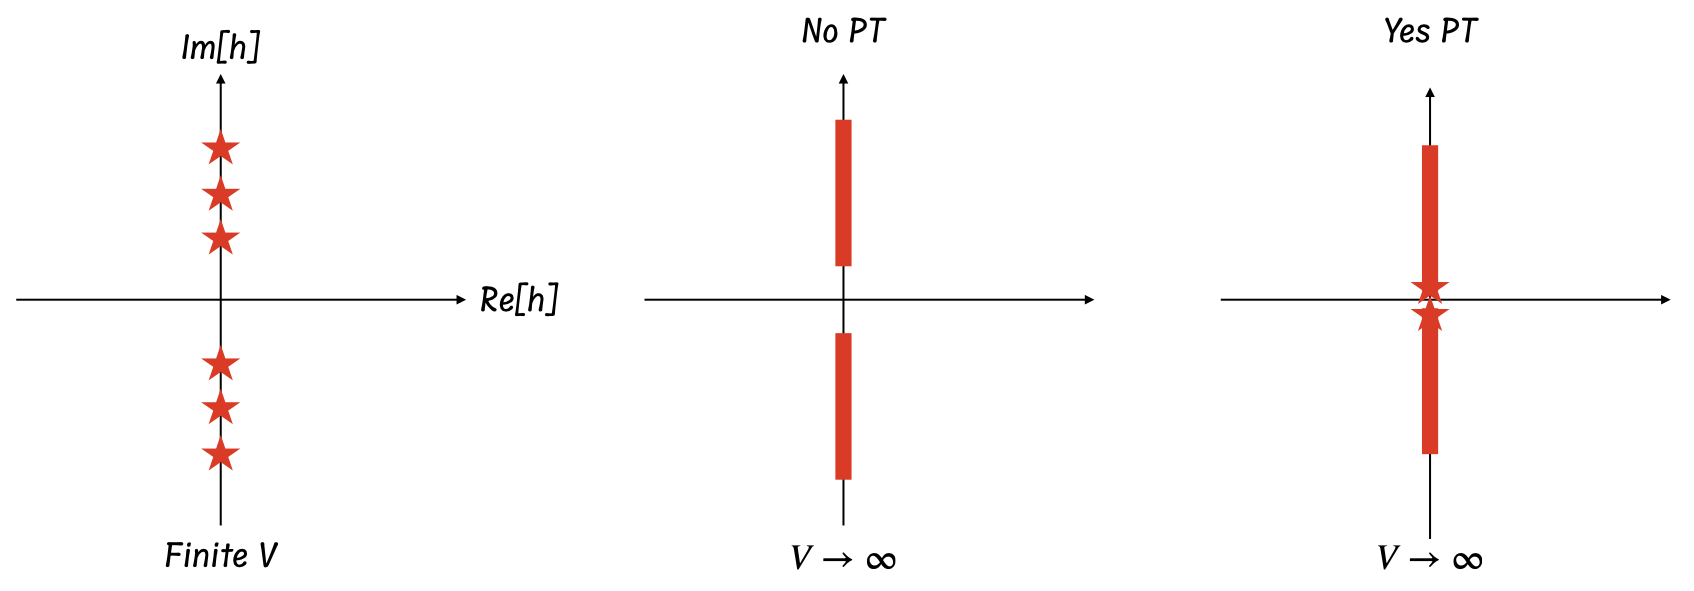
\includegraphics[scale=0.25]{LYE.png}
    \caption{Existence of phase transition}
    \label{fig:LYE}
\end{figure}

\begin{figure}
    \centering
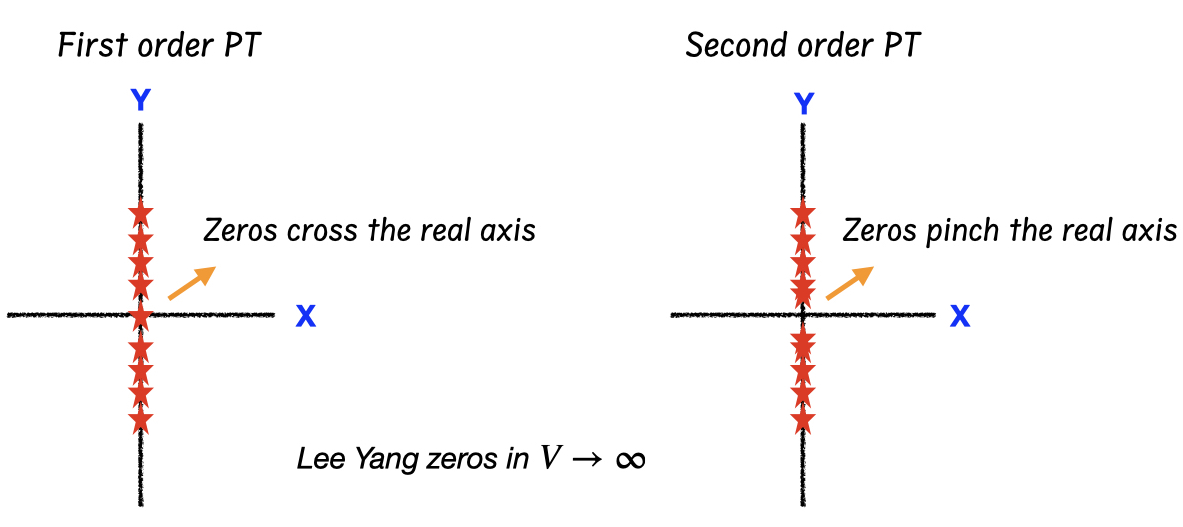
\includegraphics[scale=0.3]{LYEVinft.jpeg}
    \caption{Order of phase transition}
    \label{fig:LYEVinft}
\end{figure}

To remind ourselves again, we are interested in the zeros of the partition function, since these become singularities of thermodynamic potenitals. Looking at Eq.~\ref{eq:LYZ}, we can make some observations,

\begin{enumerate}[i]
    \item In a finite volume, the grand canonical partition functions as written in Eq.~\ref{eq:LYZ} is a \emph{finite} polynomial in the fugacity variable $z$.
    \item For any real parameter $T,\mu$, \emph{all terms} in the RHS of Eq.~\ref{eq:LYZ} are strictly positive. 
    \item Any finite polynomial with strictly positive coefficients can only have \emph{complex} roots. 
    \item These roots must come with their \emph{complex conjugate} pairs, in order to keep the partition function real.
    \item The location of the roots depends on temperature, since the coefficients and the variable of expansion $z$ depend on $T$.
\end{enumerate}

\noindent \emph{The following discussion regarding analogy of the Lee-Yang zeros to 2D electrostatics is taken from the second reference pointed to below and gives us a very nice physical picture of the partition function zeros.}

\subsection{Location of the phase transition point}
After establishing that the partition function is a polynomial in fugacity, let us write it in terms of it's roots ,
\begin{equation}
Z_{GC}^V(T, z) = \xi \prod_{i=1}^{M} \left( 1 - \frac{z}{z_i(T)} \right)
\end{equation}
where $\xi$ is some constant that can be dropped for simplicity. In the following, we will focus on  pressure at a fixed volume $P_V = -F/V$, where $F = -k_B T \ln Z^V_{GC}$, 
\begin{equation}
    P_V(z) = k_B T \frac{1}{V} \sum_{i=1}^{M} \ln \left( 1 - \frac{z}{z_i(T)} \right)
    \label{eq:PresV}
\end{equation}

Note that $P_V(z)$ is analytic in the entire complex $z$ plane except at the points $z_i$, or the Lee-Yang zeros. Further, since the number of these zeros increases with increasing volume, let us assume that they accumulate \emph{in a certain region} $\mathcal{C}$ in the complex $z$ plane with a \emph{density} given by $\rho(z)$, such that $\rho(z) = 0$ if $z \notin \mathcal{C}$. Since $\rho(z)$ is a density, it is real valued, positive ad well defined in $\mathcal{C}$. Moreover, since the roots appear in complex conjugate pairs across the $x$ axis (real $z$ axis), we have $\rho(z) = \rho(z^*)$. This means that the region of accumulation $\mathcal{C}$ is symmetric w.r.t. the real axis.

Now that we have defined the density of zeros $\rho(z)$, one can define the thermodynamic limit (since this is where non-analyticities show up) of the complex pressure defined in Eq.~\ref{eq:PresV} as follows,

\begin{equation}
    P(z) = \lim_{V \to \infty} P_V(z)  = k_B T \int dz' \rho(z') \ln \left( 1 - \frac{z}{z'} \right)
\end{equation}

where $z'$ is a \emph{real} parameter that defines how we move along our curve $\mathcal{C}$, where all the zeros accumulate. Since $z$ on the other hand is free to take any value in the complex plane, $P(z)$ is a complex function which can be written as $P(z) = \phi(z) + i \psi(z)$ with,

\begin{align}
    \phi(z) &= \frac{1}{k_B T} \text{Re} P(z) = \int dz' \rho(z') \ln \left| 1 - \frac{z}{z'} \right| \nonumber \\
    \psi(z) &= \frac{1}{k_B T} \text{Im} P(z) = \int dz' \rho(z') \arg \left( 1 - \frac{z}{z'} \right)
\end{align}

\noindent From the equation for $\phi(z)$, we can immediately recognize why this is basically a \textbf{$2$D electrostatics problem}! In two dimensions the electric field falls off like $\frac{1}{|\Vec{r} - \Vec{r'}|}$ and the potential goes like $\ln | \Vec{r} - \Vec{r'} |$. In other words, $\ln |z|$ is the Green's function of the two-dimensional Laplacian $\Delta = \partial^2_x + \partial^2_y$.

\noindent This analogy is very useful because it allows us to view $\mathcal{C}$ as a curve of charges which separates our complex $z$ plane into two parts. The electrostatic potential $\phi(z)$ is continuous everywhere in this plane, but the electric field intensity $\nabla \phi(z)$ is discontinuous on $\mathcal{C}$! Let $\phi_{1,2} (z)$ denote the two analytic expressions for the potential in the two regions. \footnote{Of course depending on the shape of $\mathcal{C}$, there can be more regions, but for simplicity we assume two in this discussion}  

A \textbf{phase transition} is set to occur if this curve intersects the real axis. If the point of intersection is $z_0$, then we have from continuity of the potential and hence the pressure,

\begin{equation*}
    Re P_1(z_0) = Re P_2(z_0)
\end{equation*}

\subsection{Nature of the transition from Lee-Yang zeros}
After establishing the condition for the phase transition to occur, we need to consider if the properties of the of the distribution of zeros give us the \emph{nature} of the phase transition. It will be shown below that it is indeed possible to determine the nature of the phase transition by analysing the behaviour of the density of zeros at the transition point. 

In order to show this we will consider $\mathcal{C}$ to be a smooth curve, parameterized by a real parameter $s$, such that $s=0$ at $z=z_0$. Further, the density of zeros becomes a \emph{line} density given by $\lambda(s)$. The vectors tangent and normal to the curve $\mathcal{C}$ are given by $\hat{t}$ and $\hat{n}$ respectively. We already saw that the real part of the pressure is continuous at $z_0$. The imaginary part part of the pressure can be related to the density of zeros again using the electrostatic analogy as follows.

We know that the electric field is discontinuous at $\mathcal{C}$,

\begin{equation}
\frac{1}{2\pi} [\nabla \phi_2(z) - \nabla \phi_1(z)] \cdot \hat{n} \bigg|_{C} = \lambda(s)
\end{equation}

But $P_1(z)$ and $P_2(z)$ are analytic functions in their own domains, hence we can use Cauchy-Riemann conditions to write,

\begin{equation}
\nabla \phi_{1,2}(z) \cdot \hat{n} \bigg|_{C} = \nabla \psi_{1,2}(z) \cdot \hat{t} \bigg|_{C}
\end{equation}

where \begin{equation}
\psi_{1,2}(z) = \frac{1}{k_B T} \text{Im} P_{1,2}(z)
\end{equation}

Since $\hat{t} = \hat{t}(s)$ is the tangent vector along the curve which is parameterized by $s$, we can write,
\begin{equation}
    \lambda(s) = \frac{1}{2\pi} \frac{d}{ds} [ \psi_2(z) - \psi_1(z) ] \bigg|_{C} = \frac{1}{2\pi k_B T} \frac{d}{ds} [ \text{Im} P_2(z) - \text{Im} P_1(z) ] \bigg|_{C}
\end{equation}

At $z=z_0$, we have,
\begin{equation}
    \lambda(0) = \frac{1}{2\pi k_B T} \frac{d}{ds} [ \text{Im} P_2(z) - \text{Im} P_1(z) ] \bigg|_{z=z_0}
    \label{eq:discImP}
\end{equation}

In order to properly justify the existence of the second order phase transition, we should study the Taylor expansion of the pressure around $z_0$ and from that determine the equation of the curve $\mathcal{C}$. However, without going into that much details and just from Eq.~\ref{eq:discImP} we can say the following,

\begin{itemize}
    \item If $\lambda(0) \neq 0$, then the pressure has a discontinuity in it's first derivative and hence a first-order phase transition is set to occur.
    \item If $\lambda(0) = 0$, the first derivative is continuous. If one studies the shape of the curve one can easily see that although the first derivative of the pressure is continuous, the density of zeros can have a \emph{cusp} at the $z_0$, leading to a second order phase transition.
    \item Even higher order transitions can be seen to happen depending on which derivative of the pressure is discontinuous.
\end{itemize}

\section{Ising model and Circle theorem}

Recall from last time that we can exactly solve for the partition function in $1$D using the transfer matrix formalism to arrive at

\begin{align}
    Z^{(P)}_N &= \text{Tr} \, T^N \nonumber \\
    &= \lambda^N_+ + \lambda^N_-
\end{align}

Where we computed the eigenvalues to be given by,

\begin{equation}
    \lambda_{\pm} = e^K \, \left[ \cosh{h} \pm \sqrt{\sinh{h}^2 + e^{-4K}} \right] \label{eq:roots}
\end{equation}

In order to find the Yang-Lee zeros of this theory, we need to find the values of $T,h$ such that $Z_N = \lambda^N_+ + \lambda^N_- = 0$, since $\lambda_{\pm} \neq 0$, the only other solutions to this equation are when $\lambda_+ = (-1)^{\frac{1}{N}} \lambda_-$. Using $-1 = e^{i(2*n-1)\pi}$ we get,

\begin{align}
    \lambda_+ =  e^{i \frac{2n-1}{ N}\pi} \lambda_-   \,\,\,,\,\,\, n = 1,2... \, N
\end{align}

In order to solve the above equation, multiply the RHS and LHS by $e^{i \frac{2n-1}{2 N}\pi}$, and expand the exponential in terms of sine \& cosine to get,

\begin{align}
    \cos{\left(\frac{2n-1}{2 N}\pi \right)} \sqrt{\sinh{h}^2 + e^{-4K}} = i \sin{\left(\frac{2n-1}{2 N}\pi \right)} \cosh{h}
\end{align}

Squaring the equation above and expressing hyperbolic sine on the LHS in terms of hyperbolic cosine and on the RHS expressing the sine in terms of cosine gives us,

\begin{align}
    \cosh^2{h} =  \cos^2{\left(\frac{2n-1}{2 N}\pi \right)} \left(1 - e^{-4 K} \right)
\end{align}

Looking at the equation above one can immediately see that there are no solution for real values of the external magnetic field $h$. In order to verify this you can plot the functions and see that they don't intersect for any real $h,K$. Let us turn to $h_n = i \theta_n$, with $\theta_n \in \mathbb{R}$. This gives us solutions,

\begin{align}
    \cos{\theta_n} = \sqrt{1 - e^{-4 K }}\cos{\left(\frac{2n-1}{2 N}\pi \right)}
\end{align}

One can use some plotting software to see how these zeros appear in the complex $h$ plane. See Fig. \ref{fig:1DIsing}

\begin{figure}[ht]
    \centering
    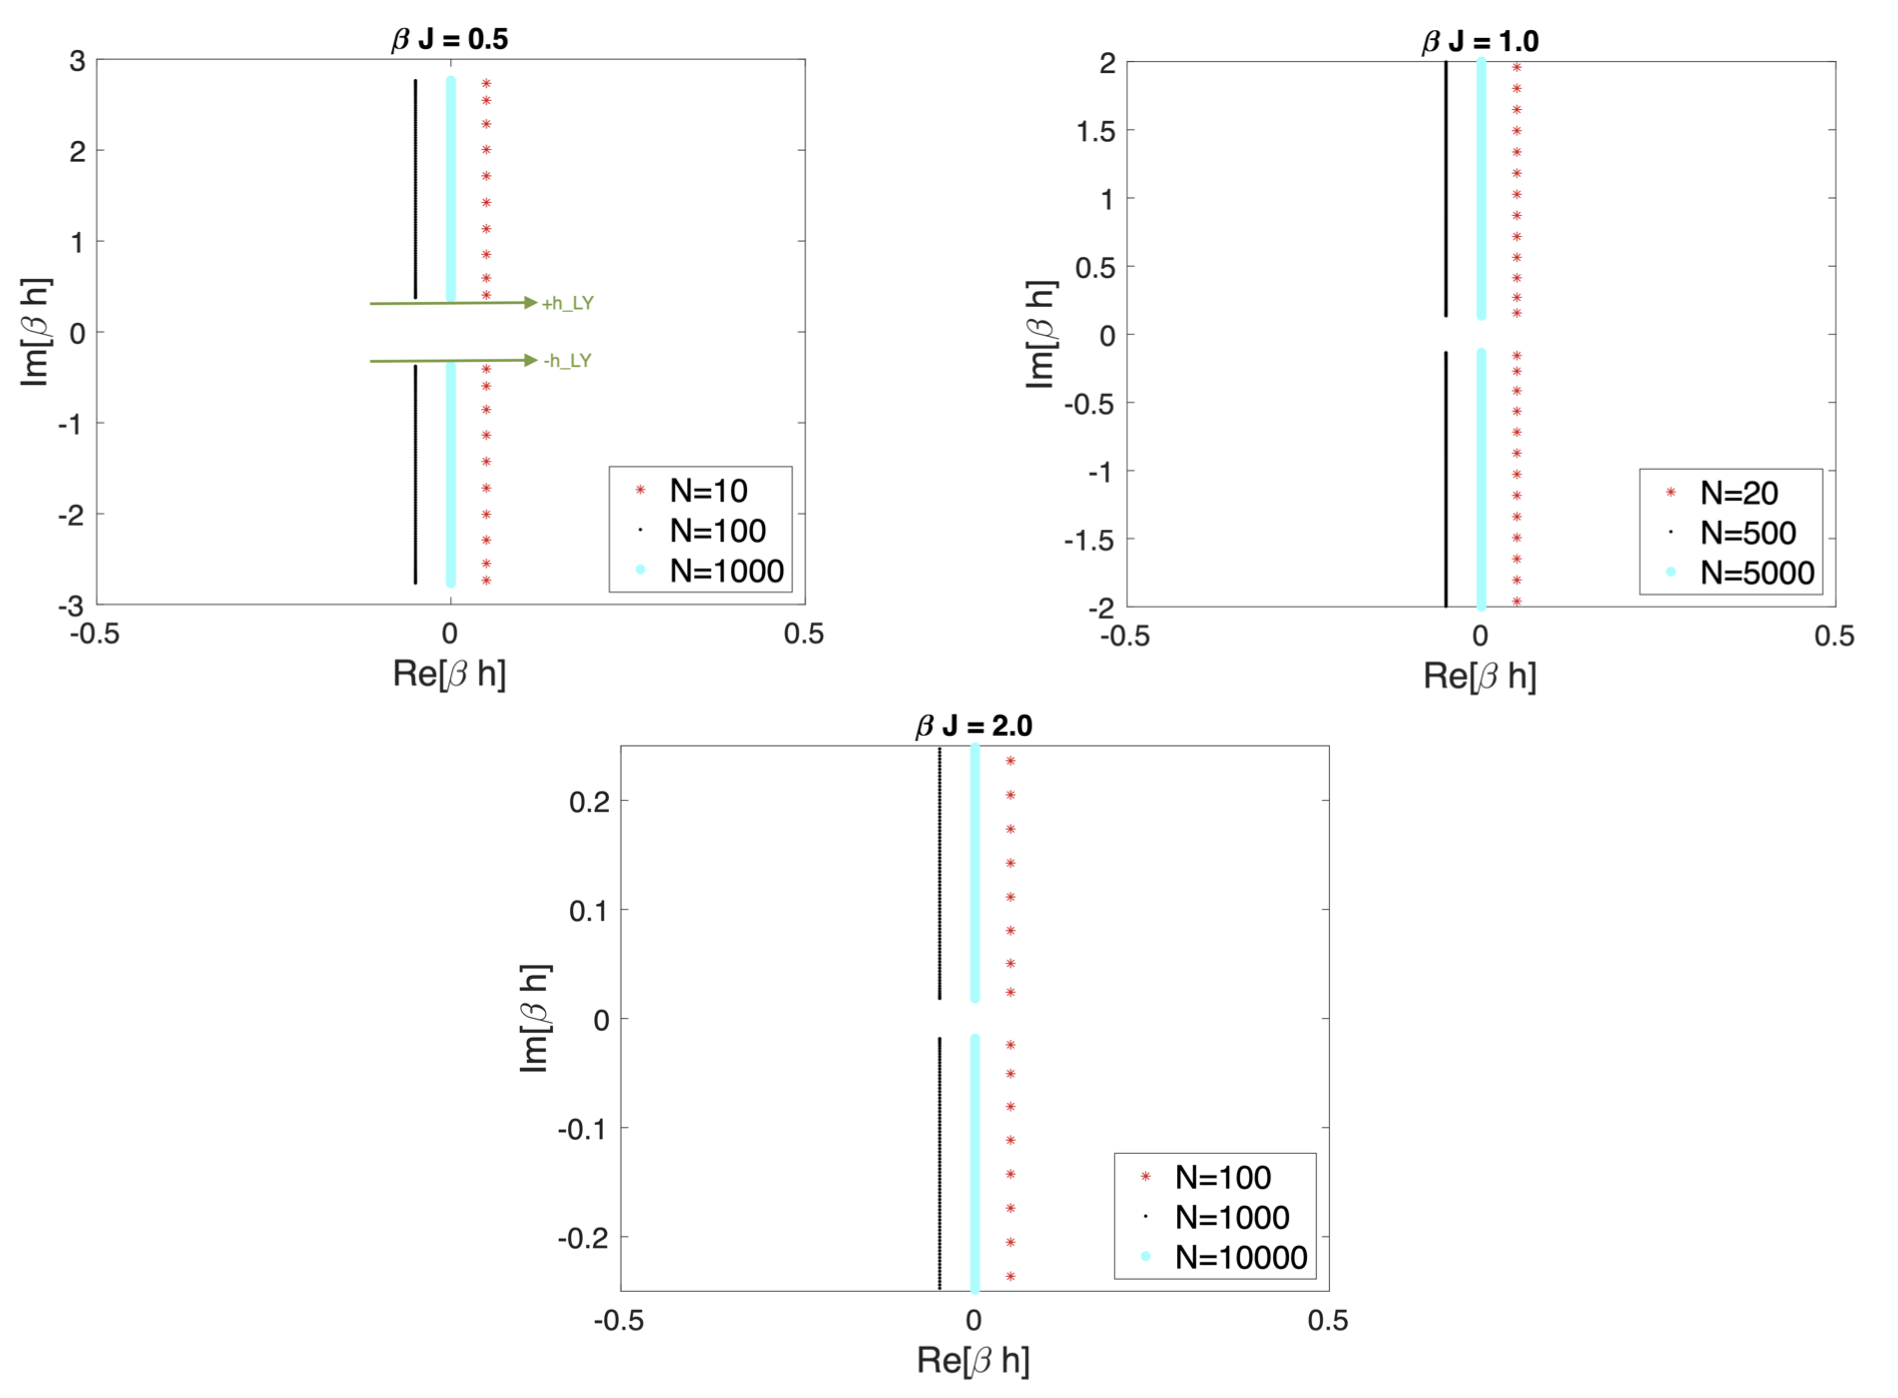
\includegraphics[scale=0.2]{1DIsing.png}
    \caption{Lee Yang zeros for 1D Ising model}
    \label{fig:1DIsing}
\end{figure}

\textbf{Some observations:}
\begin{itemize}
    \item The number of zeros increase with the number of lattice sites, the closest zero $\theta_0$ is determined by the temperature $T$.
    \item At any finite temperature, $e^{-4K} > 0$, this means, $\cos{\theta_n} \leq \left(1-e^{-4K}\right) < 1$, $\theta_n$ can never be 0! Hence the $1$D Ising model with ferromagnetic interactions doesn't have a phase transition.
\end{itemize}

\section{Literature : References and further reading}

Most of these notes are adapted from the original Yang-Lee paper and a relatively recent review paper:
\begin{enumerate}[i]
    \item Statistical Theory of Equations of State and Phase Transitions. I. Theory of Condensation, C. N. Yang and T. D. Lee Phys. Rev. 87, 404 (1952)
    \item STATISTICAL MECHANICS OF EQUILIBRIUM AND NON-EQUILIBRIUM PHASE TRANSITIONS: THE YANG-LEE FORMALISM, I. Bena, M. Droz and A. Lipowski (2005)
\end{enumerate}

\end{document}